\documentclass[spanish]{beamer}
\usepackage[ansinew]{inputenc} % Acepta caracteres en castellano
\usepackage[spanish]{babel}    % silabea palabras castellanas
\usepackage{amsmath}
\usepackage{mathtools,cancel} % cancela con una flecha \cancelto{0}{XXXX}
\renewcommand{\CancelColor}{\color{red}} %change cancel color to red
\usepackage{amsfonts}
\usepackage{amssymb}
\usepackage{dsfont}
\usepackage{graphicx}
\usepackage{geometry}
\usetheme{Madrid}
\usecolortheme{beaver}
\usepackage{textpos}
% Logo  en el comienzo 
\addtobeamertemplate{frametitle}{}{%
\begin{textblock*}{100mm}(.85\textwidth,-1cm)
{\includegraphics[height=0.4in, keepaspectratio=true]{/Users/luisnunez/Dropbox/MisDocumentos/UIS/UISImagenInstitucional/UISLOGO.png}}
\end{textblock*}}

\begin{document}

\title{\textbf{�rbitas y fuerzas centrales} }
\author[L.A. N��ez]{\textbf{Luis A. N��ez}}  
\institute[UIS]{\textit{Escuela de F�sica, Facultad de Ciencias, } \\
\textit{Universidad Industrial de Santander, Santander, Colombia } \\
{\includegraphics[height=0.4in, keepaspectratio=true]{/Users/luisnunez/Dropbox/MisDocumentos/UIS/UISImagenInstitucional/UISLOGO.png}}
}
\date{\today}
\maketitle


\begin{frame}
\frametitle{Agenda}
  \tableofcontents
\end{frame}


%%%%% Diapo 1
\section{Problema de dos cuerpos}
\frame{
  \frametitle{Problema de dos cuerpos 1/3}
   \begin{itemize}  
  	\item<1-> Consideremos dos part�culas $m_1$ y $m_2$ en $\mathbf{r}_1$ y $\mathbf{r}_2$, respecto a un origen $O$ de un sistema de referencia inercial. 
	\item<2-> Supongamos que las part�culas interaccionan mediante un potencial que depende solamente de sus posiciones relativas, $V\left(\mathbf{r}_1, \mathbf{r}_2\right)=V\left(\mathbf{r}_2-\mathbf{r}_1\right) $. Este sistema se conoce como el problema de dos cuerpos. 
	\item<3-> El sistema posee seis grados de libertad: tres coordenadas para $\mathbf{r}_1$ de la part�cula 1 y  tres para $\mathbf{r}_2$.
	\item<4-> Definimos el vector de posici�n del centro de masa (CM) del sistema como $\mathbf{R}=\frac{m_1 \mathbf{r}_1+m_2 \mathbf{r}_2}{m_1+m_2}$ y posici�n relativa como $\mathbf{r}=\mathbf{r}_2-\mathbf{r}_1$
	\begin{figure}[t]
		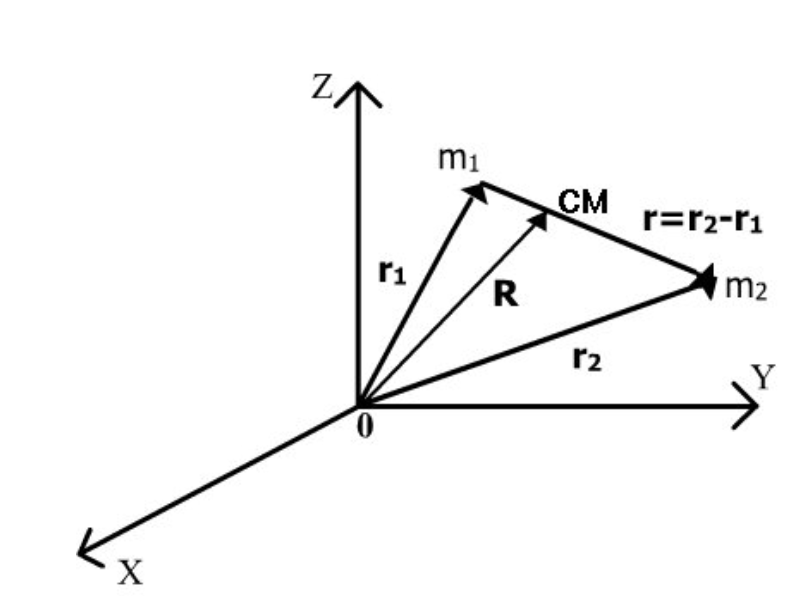
\includegraphics[width=1.7in]{Figuras/DosCuerpos.png}
   	\end{figure}
    \end{itemize}
}
%%%%% Diapo 2
%\section{Secci�n}
\frame{
  \frametitle{Problema de dos cuerpos 2/3}
   \begin{itemize}  
  	\item<1-> Las posiciones de las part�culas relativas al centro de masa son $\mathbf{r}_1^{\prime}  =\mathbf{r}_1-\mathbf{R}$ y $\mathbf{r}_2^{\prime} =\mathbf{r}_2-\mathbf{R}$
	\item<2-> Es decir: $\mathbf{r}_1^{\prime}=\mathbf{r}_1-\frac{m_1 \mathbf{r}_1+m_2 \mathbf{r}_2}{m_1+m_2}=\frac{m_2\left(\mathbf{r}_1-\mathbf{r}_2\right)}{\left(m_1+m_2\right)}=-\frac{m_2}{\left(m_1+m_2\right)} \mathbf{r}$ y 
	$ \mathbf{r}_2^{\prime}=\mathbf{r}_2-\frac{m_1 \mathbf{r}_1+m_2 \mathbf{r}_2}{m_1+m_2}=\frac{m_1\left(\mathbf{r}_2-\mathbf{r}_1\right)}{\left(m_1+m_2\right)}=\frac{m_1}{\left(m_1+m_2\right)} \mathbf{r}$
	\item<3-> La energ�a cin�tica total del sistema ser� $T=T_{\mathrm{cm}}+T_{\mathrm{rel}}$
	\item<4-> Entonces $T_{\mathrm{cm}} =\frac{1}{2} M_T \dot{\mathbf{R}}^2=\frac{1}{2}\left(m_1+m_2\right) \dot{\mathbf{R}}^2$
	\item<5-> y $T_{\mathrm{rel}} =\frac{1}{2} m_1 \dot{\mathbf{r}}_1^{\prime 2}+\frac{1}{2} m_2 \dot{\mathbf{r}}_2^{\prime 2} =\frac{1}{2} \frac{m_1 m_2^2}{\left(m_1+m_2\right)^2} \dot{\mathbf{r}}^2+\frac{1}{2} \frac{m_1^2 m_2}{\left(m_1+m_2\right)^2} \dot{\mathbf{r}}^2 =\frac{1}{2} \frac{m_1 m_2}{\left(m_1+m_2\right)} \dot{\mathbf{r}}^2$
	\item<6-> y si definimos la masa reducida, $\mu \equiv \frac{m_1 m_2}{\left(m_1+m_2\right)}$
	\item<7-> El Lagrangiano del sistema es 
	$L(\mathbf{r}, \mathbf{R}, \dot{\mathbf{r}}, \dot{\mathbf{R}}) =T-V\left(\mathbf{r}_2-\mathbf{r}_1\right) =\frac{1}{2}\left(m_1+m_2\right) \dot{\mathbf{R}}^2+\frac{1}{2} \mu \dot{\mathbf{r}}^2-V(\mathbf{r})$
	\item<8-> Los seis grados de libertad del sistema se describen mediante las componentes de los vectores $\mathbf{r}$ y $\mathbf{R}$.
    \end{itemize}
}

%%%%% Diapo 2
%\section{Secci�n}
\frame{
  \frametitle{Problema de dos cuerpos 3/3}
   \begin{itemize}  
  	\item<1-> Las componentes cartesianas de $\mathbf{R}$ son coordenadas c�clicas, lo que implica $M_{\mathrm{T}} \dot{\mathbf{R}} \equiv (m_1+m_2)\dot{\mathbf{R}}=$ cte. \\ Es decir: {\bf el momento lineal total del sistema se conserva}
	\item<2-> Como no hay fuerzas externas sobre el sistema : $\mathbf{F}_{\text {externa total }}=0 \Rightarrow \mathbf{P}_{\mathrm{T}}=M_{\mathrm{T}} \dot{\mathbf{R}}=$ cte. El centro de masa se mantiene en reposo o se mueve con velocidad constante, $\dot{\mathbf{R}}=$ $\mathbf{v}_{\mathrm{cm}}=$ cte.
	\item<3-> Existir�n tres cantidades conservadas correspondientes a las tres componentes del momento lineal total o, equivalentemente, a las tres componentes de la velocidad del centro de masa.
	\item<4-> El t�rmino $T_{\mathrm{cm}}$, la energ�a cin�tica del centro de masa es constante y se omite en el Lagrangiano, $L=\frac{1}{2} \mu \dot{\mathbf{r}}^2-V(\mathbf{r})$
	\item<5-> El problema de dos cuerpos se reduce al de una part�cula de masa $\mu$ en la posici�n relativa $\mathbf{r}(t)$ con respecto a un origen $O^{\prime}$.
	\begin{figure}[t]
		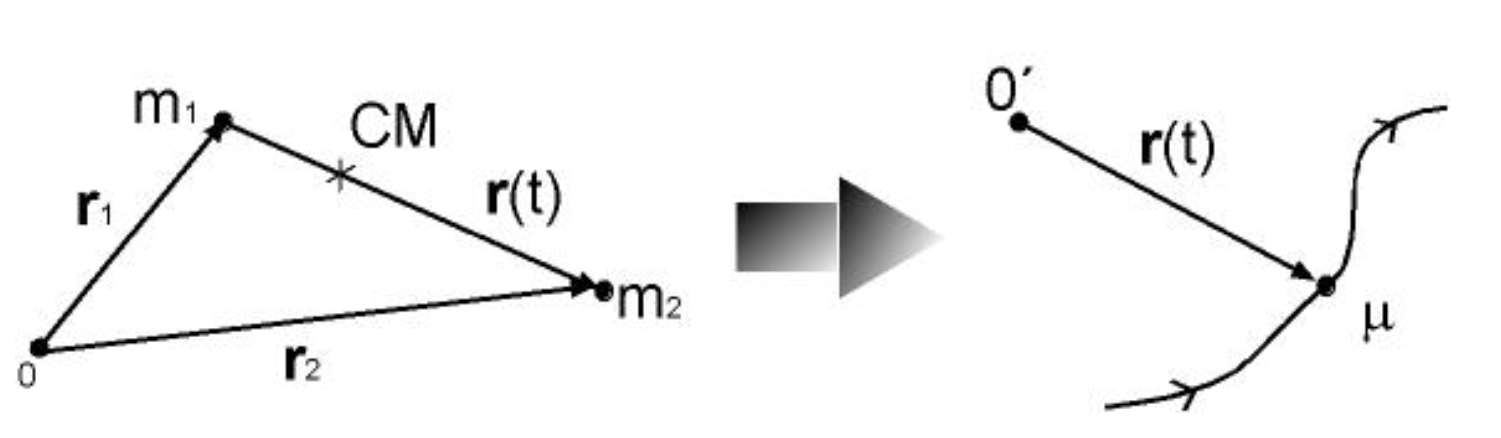
\includegraphics[width=1.7in]{Figuras/EquivalenciaDosCuerpos.png}
   	\end{figure}

    \end{itemize}
}

%%%%% Diapo 2
\section{Secci�n}
\frame{
  \frametitle{T�tulo transparencia}
   	\begin{itemize}  
  \item<1-> 
    \end{itemize}
}
  
\end{document}
%%%%% Diapo 2
\section{Secci�n}
\frame{
  \frametitle{T�tulo transparencia}
   	\begin{itemize}  
  \item<1-> 
    \end{itemize}
}
%%%%% Diapo 2
\section{Secci�n}
\frame{
  \frametitle{T�tulo transparencia}
   	\begin{itemize}  
  \item<1-> 
    \end{itemize}
}
%%%%% Diapo 2
\section{Secci�n}
\frame{
  \frametitle{T�tulo transparencia}
   	\begin{itemize}  
  \item<1-> 
    \end{itemize}
}
%%%%% Diapo 2
\section{Secci�n}
\frame{
  \frametitle{T�tulo transparencia}
   	\begin{itemize}  
  \item<1-> 
    \end{itemize}
}
